\documentclass[aspectratio=169]{beamer}
\usepackage{tikz}
\usepackage{subcaption}
%\usepackage{helvet} % Sets font to Helvetica, similar to the image's sans-serif font
\usefonttheme{professionalfonts}
\usepackage{newtxtext} % Loads the Times-like text font
\usepackage{newtxmath} % Loads the matching math font
\renewcommand{\familydefault}{\sfdefault}
\usepackage{pgfpages}
\setbeameroption{show notes on second screen=right} % Creates the double-wide PDF for Pympress
% --------------------------------
    
% Remove default Beamer navigation symbols
\setbeamertemplate{navigation symbols}{}

% Frame Title Styling
\setbeamercolor{frametitle}{fg=black}
\setbeamertemplate{frametitle}{
    \vspace{1.8cm} % Pushes the title down so it clears your department header
    \begin{beamercolorbox}[wd=\textwidth, left]{frametitle}
        \usebeamerfont{frametitle}\Large\bfseries\insertframetitle
    \end{beamercolorbox}
}
	

% --- NEW: Dynamic Source Command (Global Scope Fix) ---
\newcommand{\framesource}{} 
\newcommand{\source}[1]{\gdef\framesource{#1}}
% --------------------------------

% Custom background template for static elements
\setbeamertemplate{background}{
    \begin{tikzpicture}[remember picture, overlay]
        % 1. Top Left: Department Name
        \node[anchor=north west, align=left, font=\bfseries\large] 
            at ([xshift=0.4cm, yshift=-0.4cm]current page.north west) (dept) 
            {Department of Mathematics\\and Computer Science};
            
        % 2. Top Left: Thick black line
        \draw[line width=2pt] ([xshift=0.13cm, yshift=0.1cm]dept.south west) -- ++(2.5cm, 0);

        % 3. Bottom Left: SDU Logo
        % \node[anchor=south west] at ([xshift=-0.1cm, yshift=0.2cm]current page.south west) {\includegraphics[width=2cm]{SDU-logo-sort.jpg}};

        % 4. Right Edge: Vertical Text
        \node[anchor=center, rotate=-90, font=\bfseries\tiny] 
            at ([xshift=-0.4cm, yshift=-1.5cm]current page.north east) {sdu.dk};
        \node[anchor=center, rotate=-90, font=\bfseries\tiny] 
            at ([xshift=-0.4cm, yshift=-3.5cm]current page.north east) {\#sdudk};
    \end{tikzpicture}
}
% Custom footline (Draws source, then resets it)
\setbeamertemplate{footline}{
    \vspace{-1.2cm}
    \hbox{%
    \begin{beamercolorbox}[wd=\paperwidth,ht=2.25ex,dp=1ex,right]{}%
        \tiny \textit{\framesource} \hspace{0.5cm} \insertframenumber \hspace{0.8cm}
    \end{beamercolorbox}%
    }
    \vskip0.6cm%
    \gdef\framesource{} % <--- Resets the source to blank for the next slide!
}

% Adjust margins
\setbeamersize{text margin left=1cm, text margin right=1.5cm}


\begin{document}

% ---------------------------------------------------------
% NEXT SLIDE
% ---------------------------------------------------------

\begin{frame}
    \vspace{2cm} 
    \Huge \textbf{Legal Lean} \\
    \vspace{0.5cm}
    \Large Innovation project by Simon Holm, Johannes Rothe \& Andreas Bonde
    \vspace{0.8cm}

    
    \note{
        \textbf{Introduction (1 min)}
        \begin{itemize}
            \item din mor
        \end{itemize}
    }
\end{frame}


% ---------------------------------------------------------
% NEXT SLIDE
% ---------------------------------------------------------

\begin{frame}{Introduction}

    \begin{figure}[h]
    \centering
        \begin{subfigure}{.45\textwidth}
            
\includegraphics[width=0.5\textwidth]{assets/legal-lean-logo-black.png}
        \end{subfigure}
        \hfill
        \begin{subfigure}{.45\textwidth}
            \Large \textbf{FORM but for Law}
            \begin{itemize}
                \item MathLib and CSLib as gotten a lot of succes
                \item Provide a structured database for Law
                \item Provide a way for AI be trained better
            \end{itemize}
        \end{subfigure}
    \end{figure}

    \note{
        \textbf{Header}
        \begin{itemize}
            \item din mor
        \end{itemize}
    	}
\end{frame}




% ---------------------------------------------------------
% NEXT SLIDE
% ---------------------------------------------------------

\begin{frame}{Lean}

    \begin{figure}[h]
        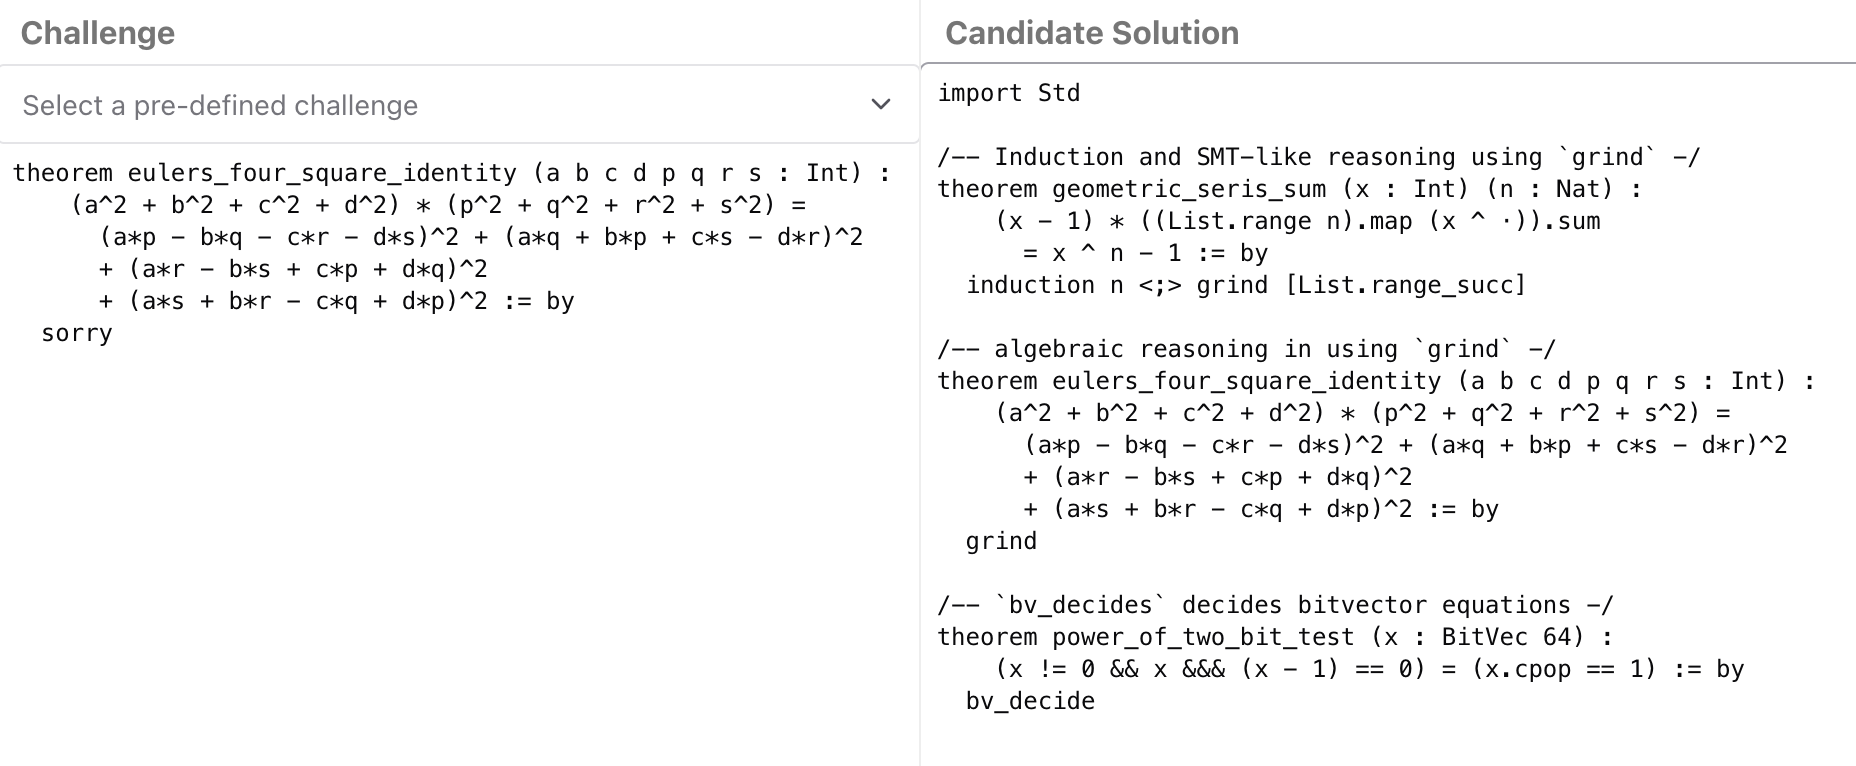
\includegraphics[width=0.7\textwidth]{assets/lean_example.png}
        \hfill
        
\includegraphics[width=0.7\textwidth]{assets/lean_example2.png}
    \end{figure}

    \note{
        \textbf{Header}
        \begin{itemize}
            \item din mor
        \end{itemize}
    	}
\end{frame}




% ---------------------------------------------------------
% NEXT SLIDE
% ---------------------------------------------------------

\begin{frame}{Lean}

    \begin{figure}[h]
        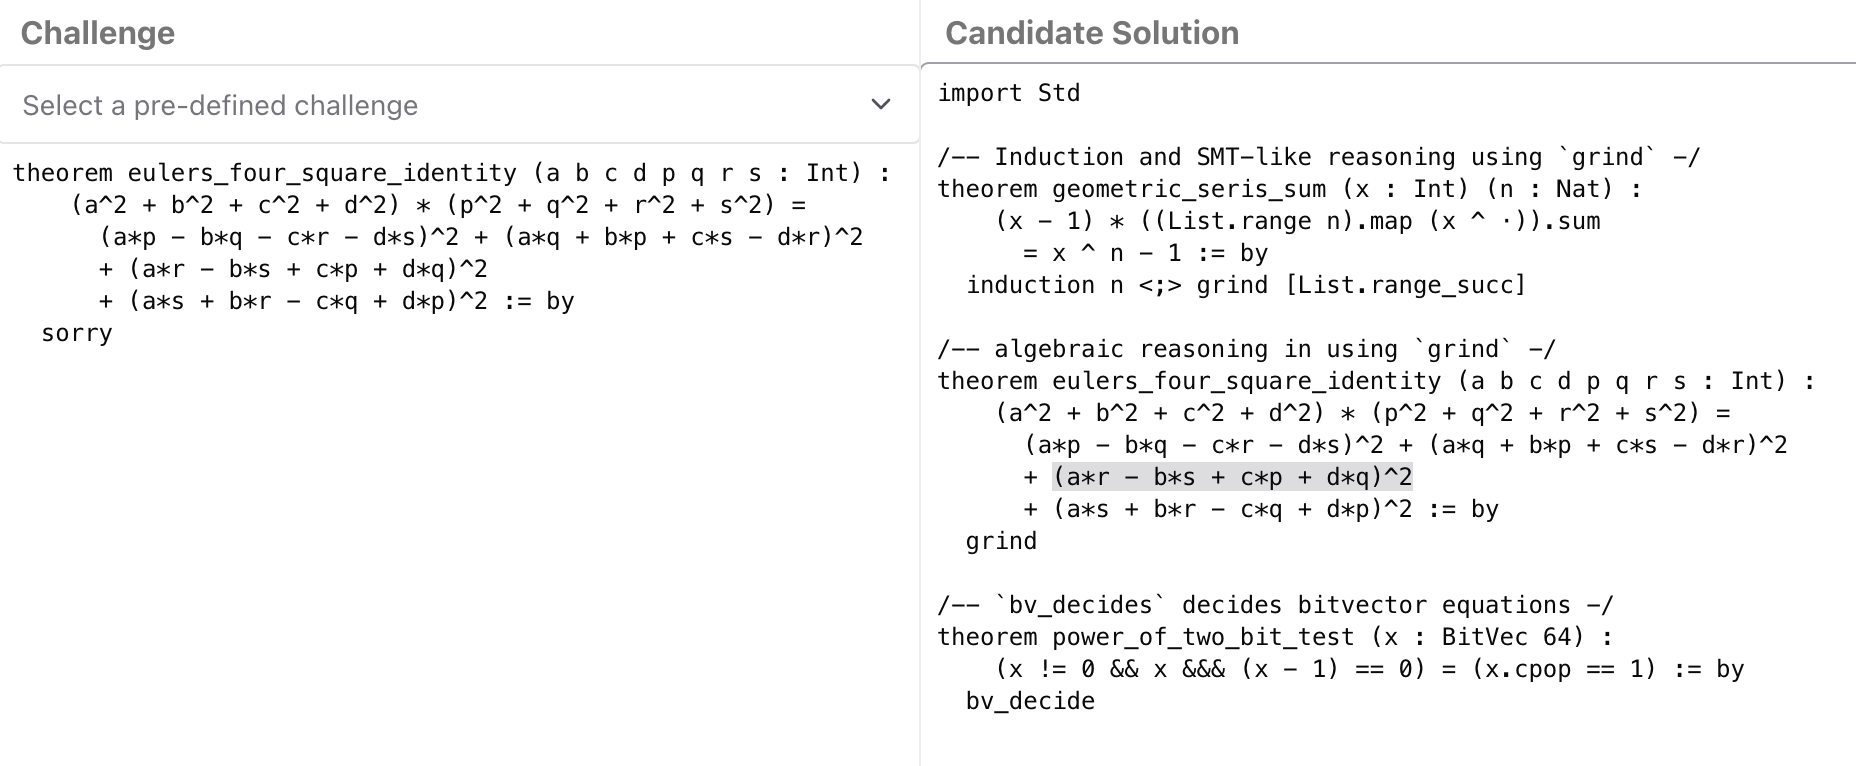
\includegraphics[width=0.7\textwidth]{assets/lean_example_fail.png}
        \hfill
        
\includegraphics[width=0.7\textwidth]{assets/lean_example_fail2.png}
    \end{figure}

    \note{
        \textbf{Header}
        \begin{itemize}
            \item din mor
        \end{itemize}
    	}
\end{frame}




% ---------------------------------------------------------
% NEXT SLIDE
% ---------------------------------------------------------

\begin{frame}{Idea Funnel}
    \begin{figure}[h]
      \centering
      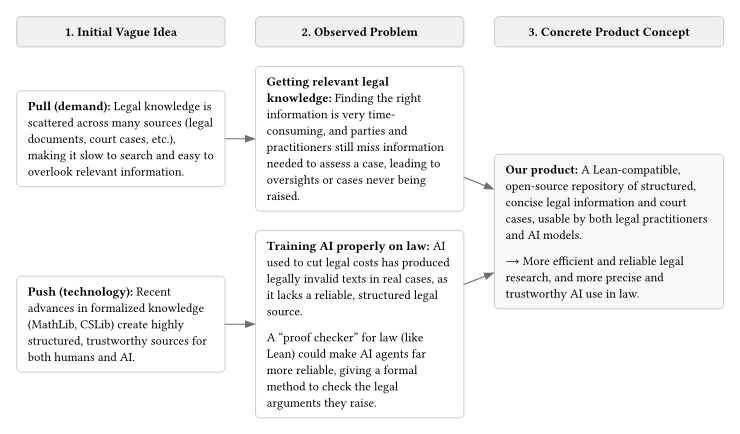
\includegraphics[width=0.7\textwidth]{assets/idea-funnel.png}
    \end{figure}
\end{frame}




% ---------------------------------------------------------
% NEXT SLIDE
% ---------------------------------------------------------

\begin{frame}{Stakeholder Mapping}
    \begin{figure}[h]
        \centering
        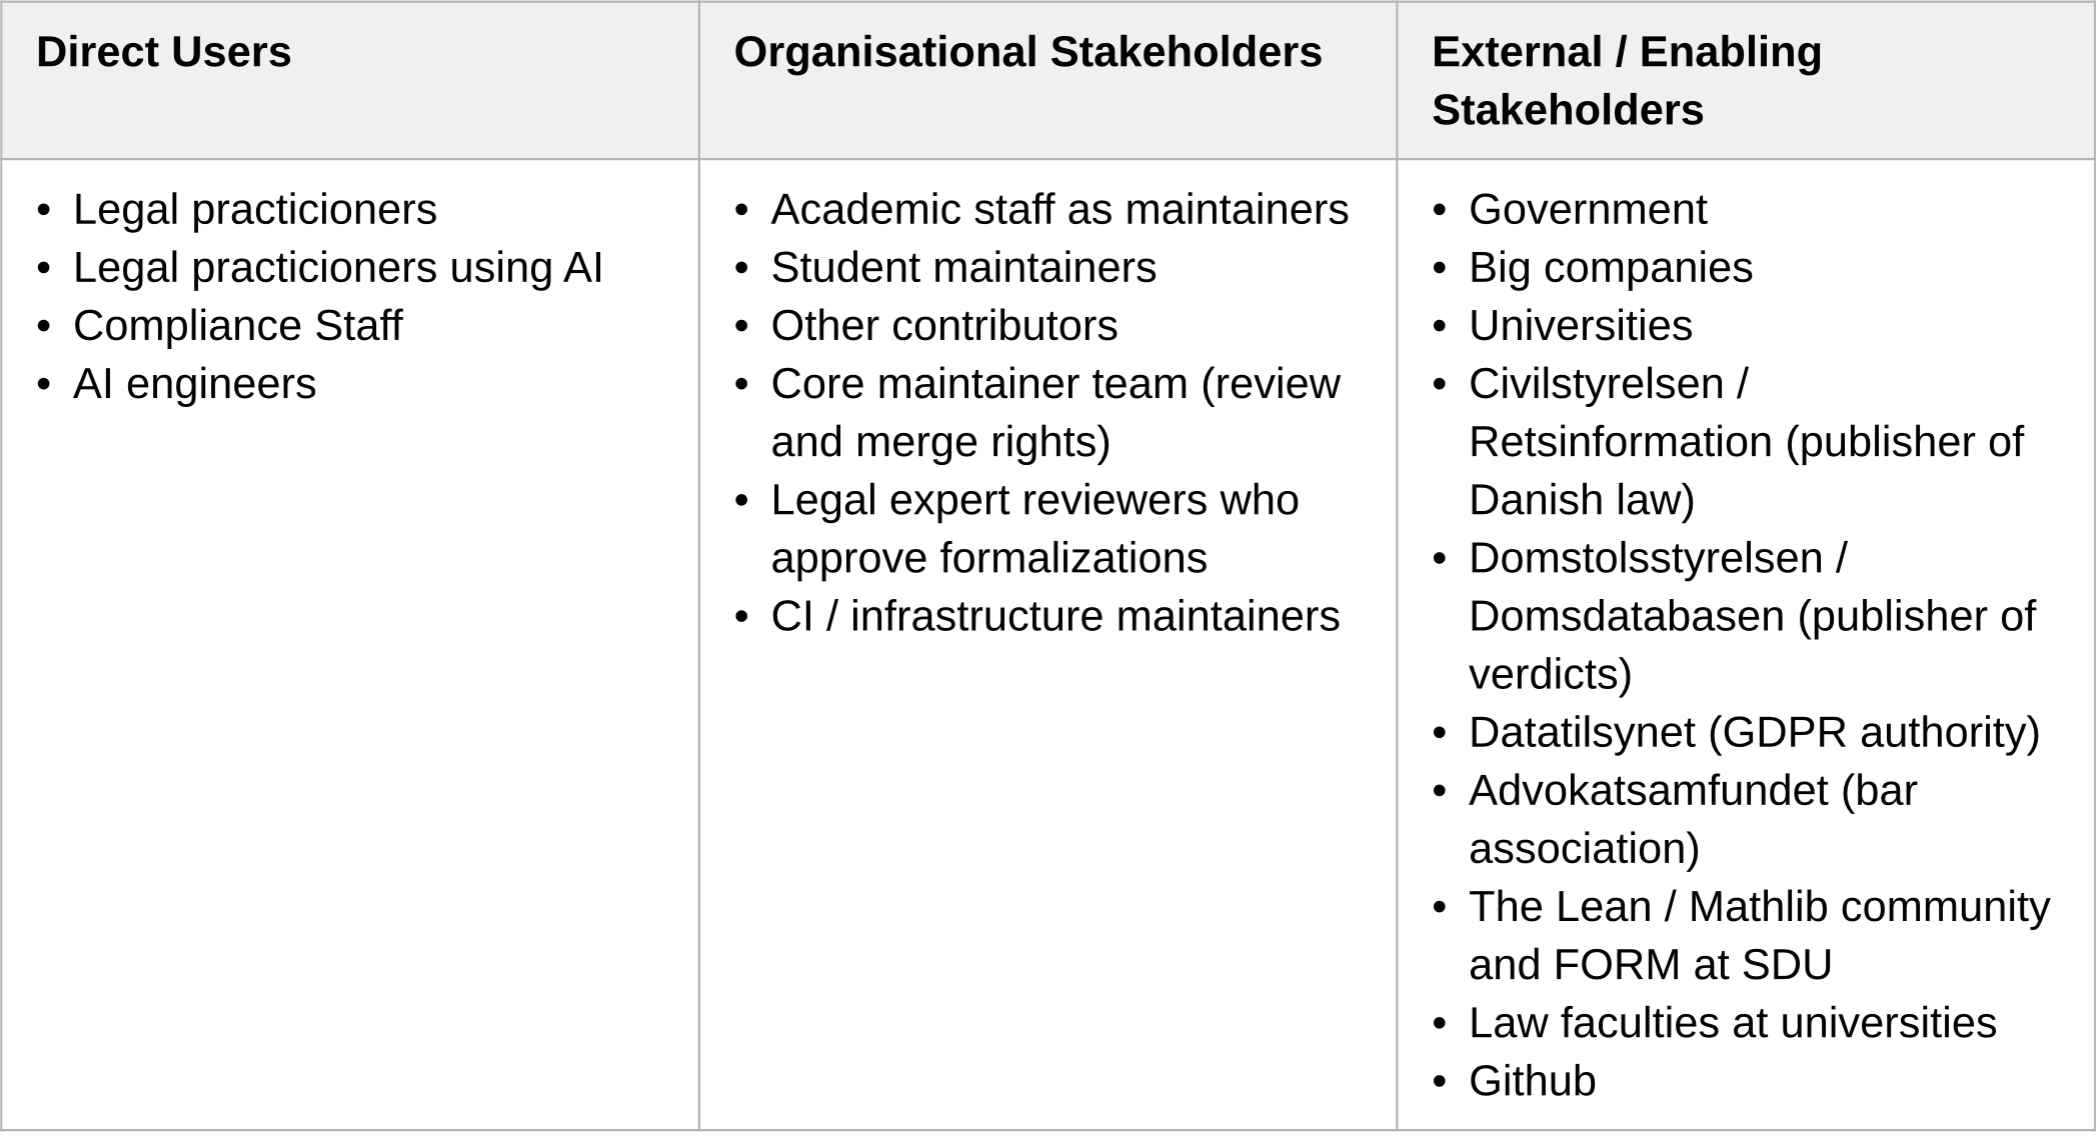
\includegraphics[width=0.7\textwidth]{assets/stakeholder_mapping.png}
    \end{figure}
\end{frame}


% ---------------------------------------------------------
% NEXT SLIDE
% ---------------------------------------------------------

\begin{frame}{SWOT Analysis}
    \begin{figure}[h]
        \centering
        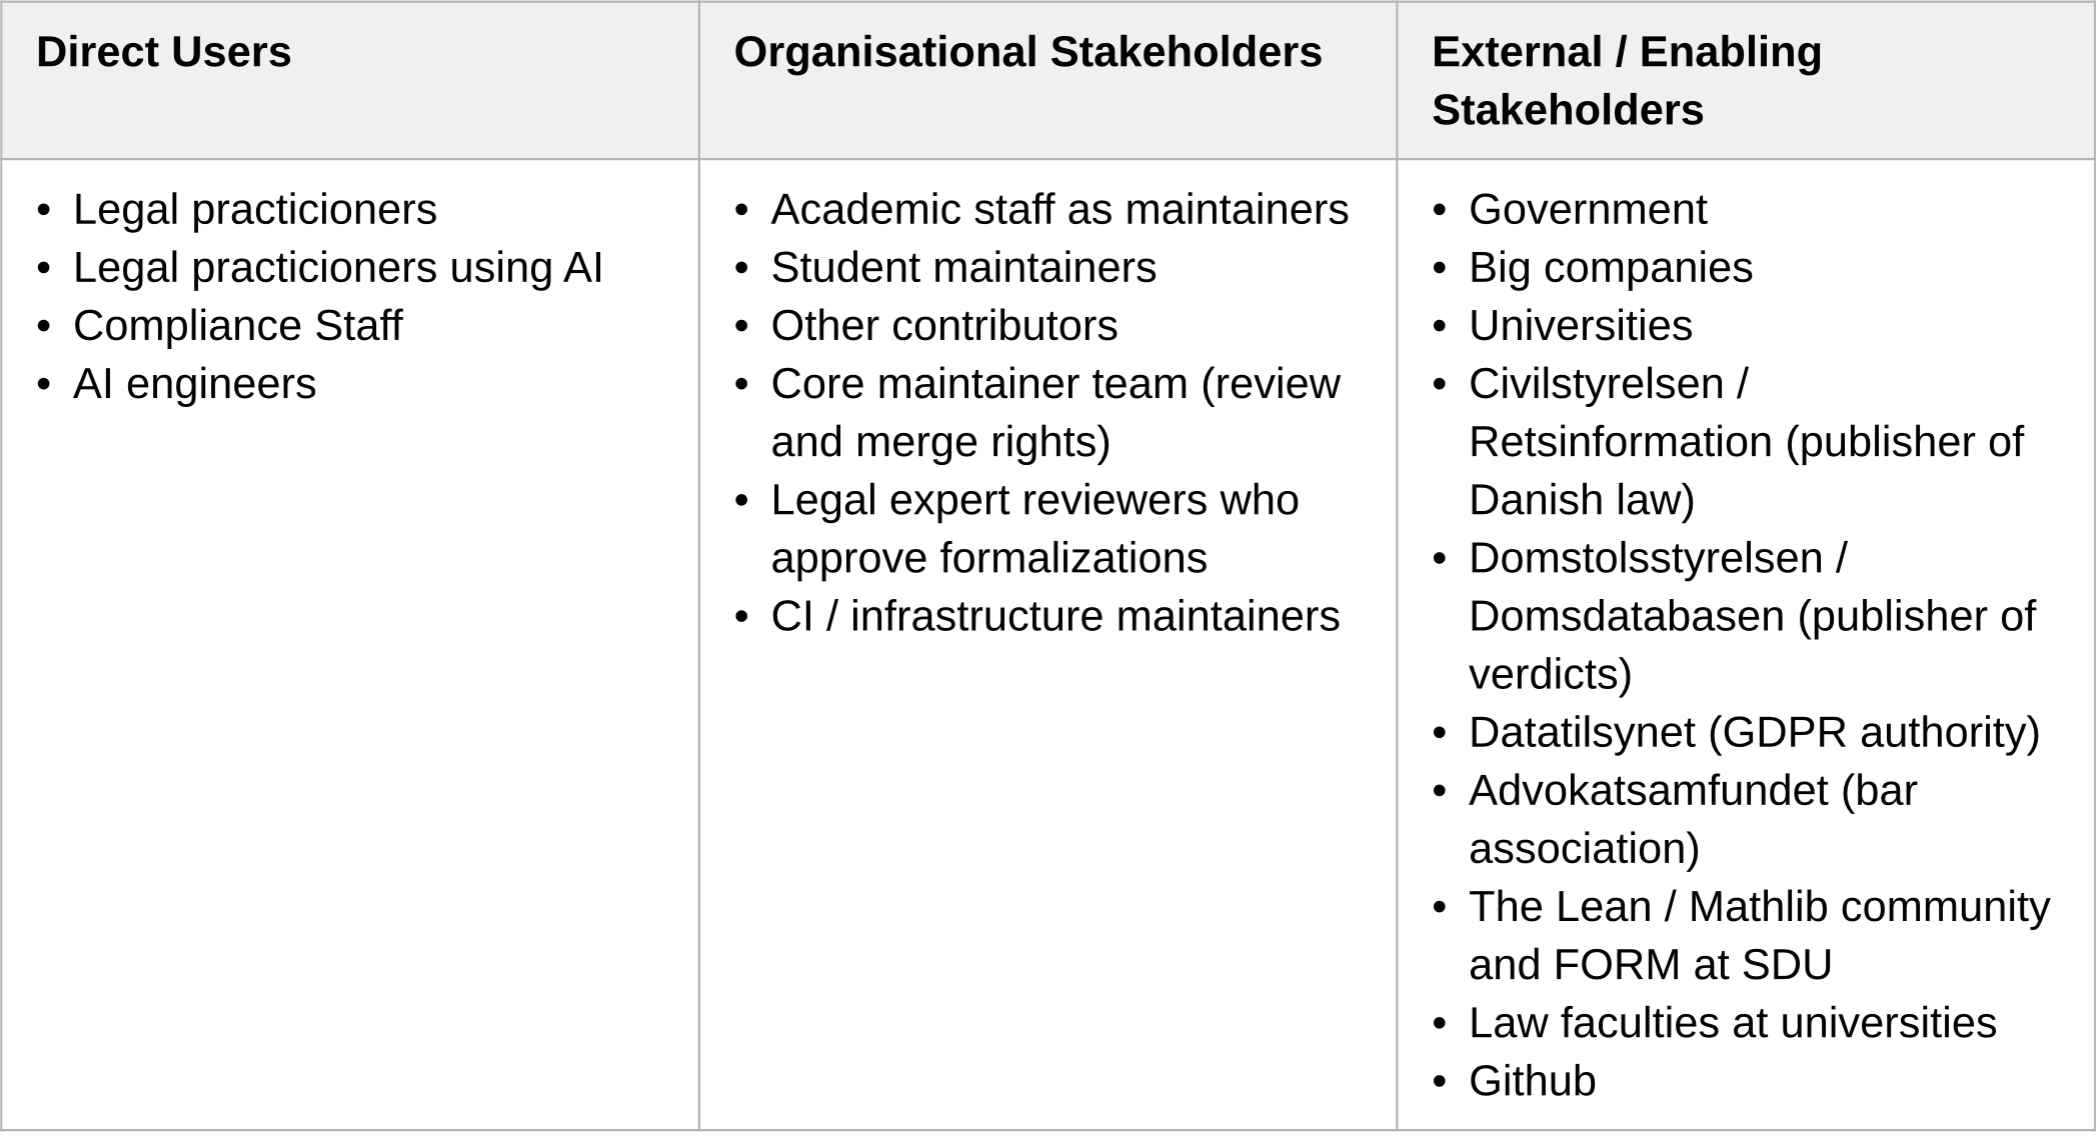
\includegraphics[width=0.7\textwidth]{assets/stakeholder_mapping.png}
    \end{figure}
\end{frame}





% ---------------------------------------------------------
% NEXT SLIDE
% ---------------------------------------------------------

\begin{frame}{Talk with a professor}
    \begin{figure}[h]
        \centering
        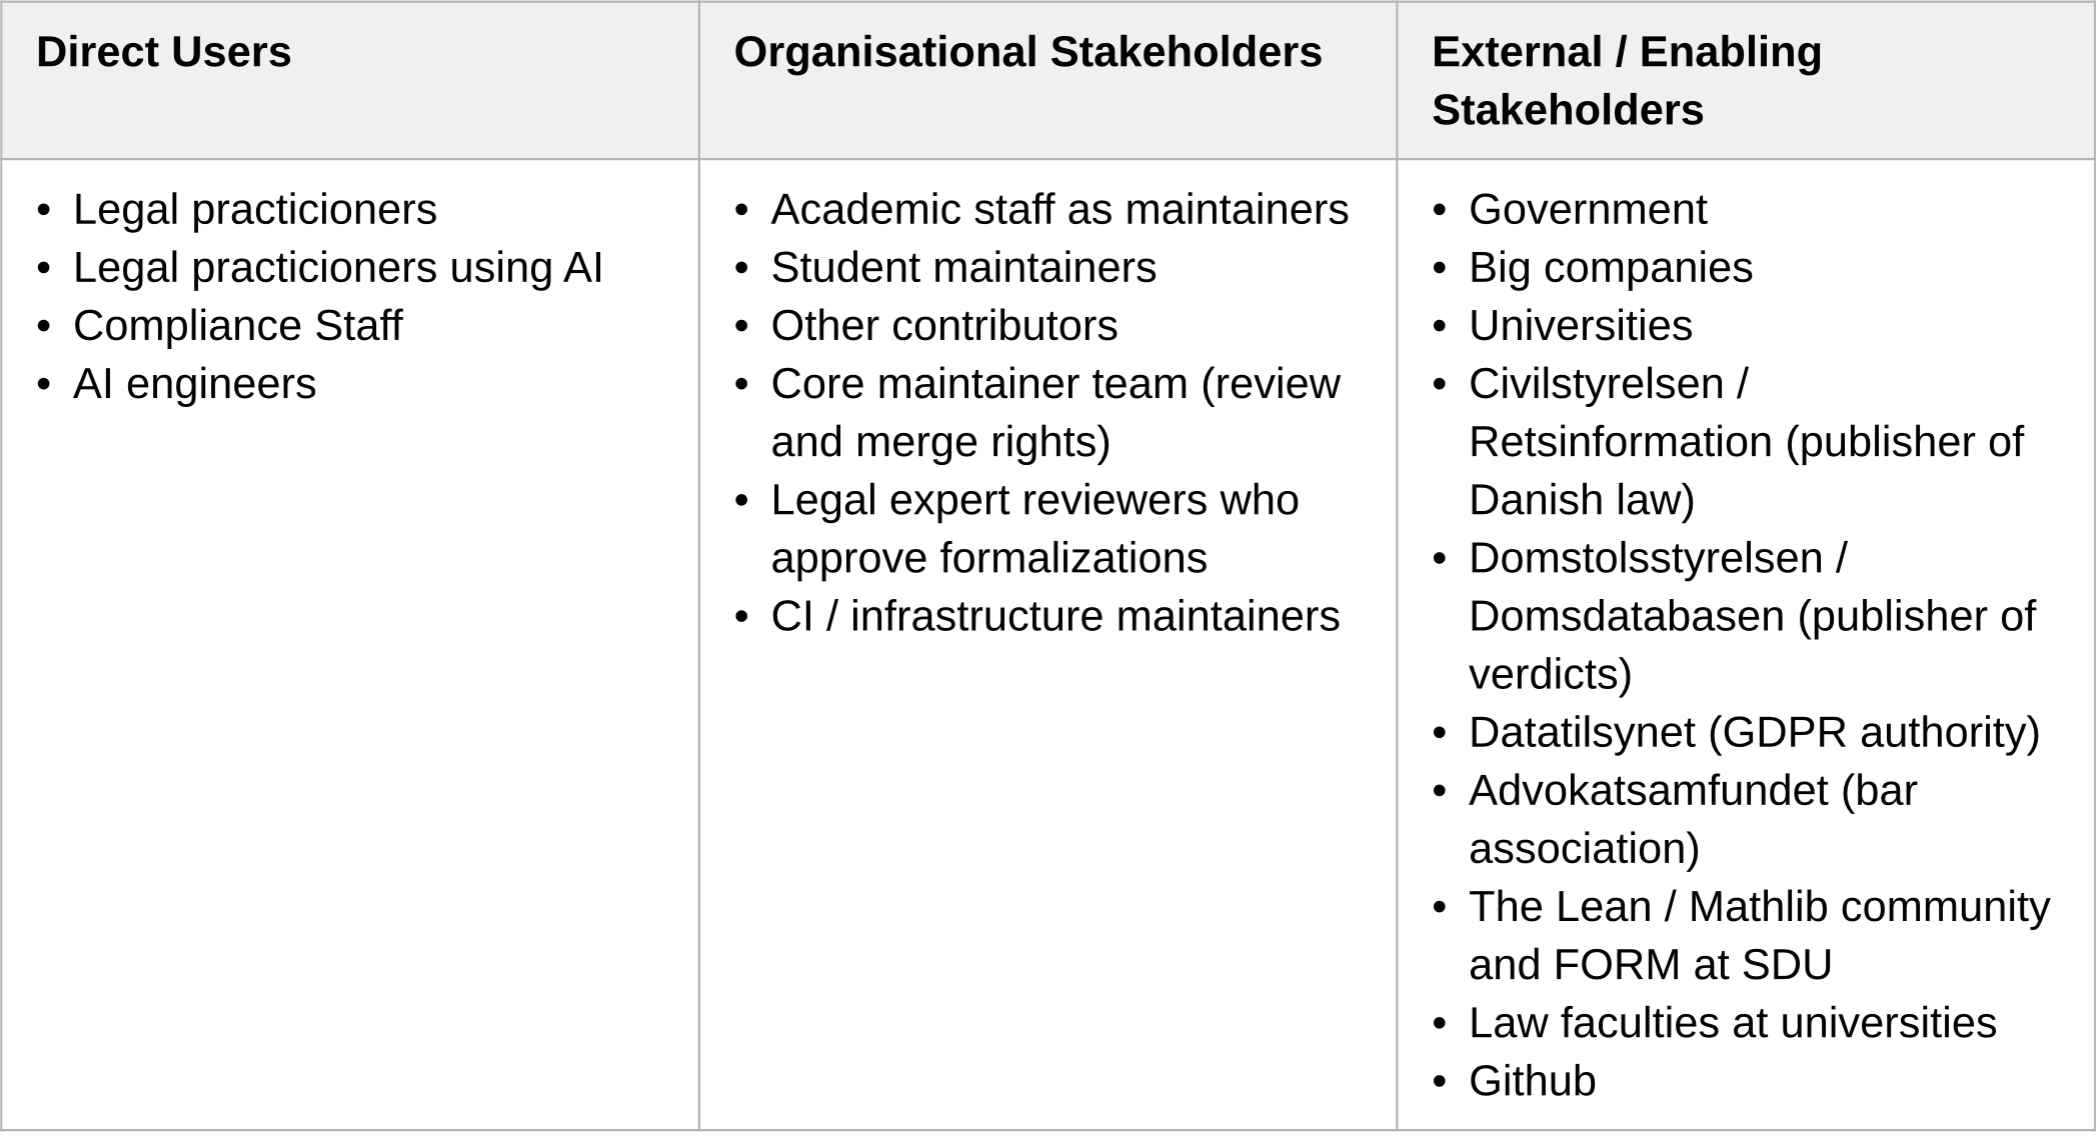
\includegraphics[width=0.7\textwidth]{assets/stakeholder_mapping.png}
    \end{figure}
\end{frame}









\end{document}



